% Standalone TikZ source for Figure 1 — A.L.F.R.E.D. system architecture.
% Compile with: pdflatex fig1_architecture.tex  -> fig1_architecture.pdf
\documentclass[border=2pt]{standalone}
\usepackage{tikz}
\usetikzlibrary{arrows.meta,positioning,calc,shapes.geometric,fit,backgrounds}

\begin{document}
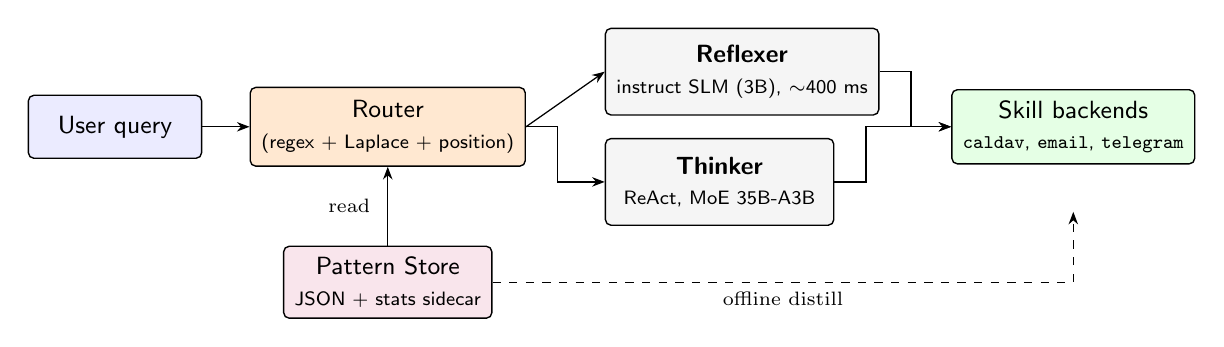
\begin{tikzpicture}[
    font=\sffamily\small,
    node distance=4mm and 6mm,
    every node/.style={align=center},
    box/.style={draw, rounded corners=2pt, minimum height=8mm, inner sep=4pt, line width=0.5pt},
    user/.style={box, fill=blue!8, minimum width=22mm},
    router/.style={box, fill=orange!18, minimum width=26mm, minimum height=10mm},
    tier/.style={box, fill=gray!8, minimum width=29mm, minimum height=11mm},
    skill/.style={box, fill=green!10, minimum width=21mm, minimum height=7mm},
    store/.style={box, fill=purple!10, minimum width=24mm, minimum height=9mm},
    >={Stealth[length=1.6mm]},
    arr/.style={->, line width=0.45pt},
    dotted-arr/.style={->, line width=0.45pt, dashed},
]

% --- User & Router ---
\node[user]   (user)   {User query};
\node[router] (router) [right=of user] {Router \\ \scriptsize (regex + Laplace + position)};

% --- Two tiers vertically stacked to the right of Router ---
\node[tier]   (refl)   [right=10mm of router, yshift=7mm]  {\textbf{Reflexer} \\ \scriptsize instruct SLM (3B), $\sim$400 ms};
\node[tier]   (think)  [right=10mm of router, yshift=-7mm] {\textbf{Thinker} \\ \scriptsize ReAct, MoE 35B-A3B};

% --- Skills (backends) ---
\node[skill]  (skills) [right=8mm of router, xshift=46mm] {Skill backends \\ \scriptsize \texttt{caldav}, \texttt{email}, \texttt{telegram}};

% --- Pattern Store (feedback) ---
\node[store]  (store)  [below=10mm of router] {Pattern Store \\ \scriptsize JSON + stats sidecar};

% --- Arrows: query path ---
\draw[arr] (user) -- (router);
\draw[arr] (router.east) -- (refl.west);
\draw[arr] (router.east) -- ++(4mm,0) |- (think.west);

% --- Tier outputs converge on Skills ---
\draw[arr] (refl.east)  -- ++(4mm,0) |- (skills.west);
\draw[arr] (think.east) -- ++(4mm,0) |- (skills.west);

% --- Pattern Store: read by router, written offline by distiller ---
\draw[arr]        (store.north) -- node[left,font=\scriptsize,xshift=-1mm]{read} (router.south);
\draw[dotted-arr] (store.east) -| node[below,font=\scriptsize,pos=0.25]{offline distill} ($(skills.south)+(0,-6mm)$);

\end{tikzpicture}
\end{document}
